\documentclass[aspectratio=169,11pt]{beamer}

\usepackage[T1]{fontenc}
\usepackage{lmodern}
\usepackage{xcolor}
\usepackage{graphicx}
\usepackage{amsmath}
\usepackage{booktabs}
\usepackage{tabularx}
\usepackage{array}

\definecolor{primary}{HTML}{1F2937}
\definecolor{accent}{HTML}{0F766E}
\definecolor{muted}{HTML}{64748B}
\definecolor{soft}{HTML}{F8FAFC}
\definecolor{warn}{HTML}{B45309}

\usetheme{default}
\usecolortheme{default}
\setbeamercolor{title}{fg=primary}
\setbeamercolor{frametitle}{fg=primary}
\setbeamercolor{structure}{fg=accent}
\setbeamercolor{block title}{fg=white,bg=primary}
\setbeamercolor{block body}{fg=primary,bg=soft}
\setbeamercolor{alerted text}{fg=warn}
\setbeamertemplate{navigation symbols}{}
\setbeamertemplate{footline}{%
  \hfill\insertframenumber/\inserttotalframenumber\hspace{2mm}\vspace{2mm}%
}
\setbeamertemplate{caption}{\raggedright\insertcaption\par}

\graphicspath{
  {../results/parameter_variants/common/}
  {../results/parameter_variants/paper_text/}
  {../results/parameter_variants/original_notebook/}
  {../results/}
}

\title{Queues under Stochastic Priority Switching}
\subtitle{Replication Results, Diagnostics, and Extensions}
\author{\small Stochastic Operations Research --- Course Project}
\date{June 2026}

\newcommand{\ok}{\textcolor{accent}{Supported}}
\newcommand{\partialok}{\textcolor{warn}{Partial}}
\newcommand{\notok}{\textcolor{warn}{Not confirmed}}
\newcommand{\code}[1]{\texttt{#1}}

\begin{document}

\begin{frame}
\titlepage
\vspace{-1em}
\begin{center}
\small Original study: Palmer, Panayidis, Knight, and Williams, JORS.
\end{center}
\end{frame}

\begin{frame}{Executive Assessment}
\small
\begin{tabularx}{\textwidth}{@{}p{0.28\textwidth}p{0.18\textwidth}X@{}}
\toprule
Experiment & Status & Evidence from current rerun \\
\midrule
Overtaking distribution, Fig.\ 5 & \partialok &
The code reproduces the comparison workflow, but the paper candidate $(3,1)$ is not the best point in this run. \\
Stability / ADF check & \partialok &
The original-notebook setting reproduces the stable/unstable split; the paper-text setting leaves the stable case inconclusive. \\
Bounded Markov approximation & \ok &
Both parameter variants converge by $b=22$, with boundary quantities below $10^{-4}$. \\
Effect of switching matrix $H$ & \partialok &
Scenarios B and C satisfy the boundary threshold; Scenario A violates the $Q(16)<0.012$ check. \\
Extensions & \ok &
Fine-grid calibration and sojourn-time variance are useful exploratory analyses, not replacements for paper metrics. \\
\bottomrule
\end{tabularx}

\vspace{0.8em}
\begin{block}{Bottom line}
The reproduction pipeline is complete and informative, but the numerical evidence should be reported as a mixed replication rather than a full success.
\end{block}
\end{frame}

\begin{frame}{Replication Architecture}
\small
\begin{columns}[T]
\column{0.48\textwidth}
\begin{block}{Inputs}
\begin{itemize}
  \item Original source code under \code{original/src}
  \item Surgery waiting-list data from the original repository
  \item Paper-text parameters
  \item Original-notebook parameter variants
\end{itemize}
\end{block}

\column{0.52\textwidth}
\begin{block}{Reproduction layer}
\begin{itemize}
  \item \code{reproduction/utils.py}: shared data, simulation, and metric helpers
  \item One script per paper experiment
  \item \code{run\_parameter\_variants.py}: paper-text and notebook runs
  \item CSV metrics plus PNG figures for auditability
\end{itemize}
\end{block}
\end{columns}

\vspace{0.8em}
\begin{center}
\footnotesize
Main result folders: \code{results/parameter\_variants/common},
\code{paper\_text}, and \code{original\_notebook}.
\end{center}
\end{frame}

\begin{frame}{Why Two Parameter Variants Were Needed}
\small
\begin{tabularx}{\textwidth}{@{}p{0.23\textwidth}p{0.23\textwidth}p{0.25\textwidth}X@{}}
\toprule
Experiment & Paper-text setting & Notebook setting & Impact \\
\midrule
Stability & $\theta_{12}=3,\theta_{21}=1$ & $\theta_{12}=2,\theta_{21}=1$ &
Notebook setting reproduces ADF split; paper-text setting does not. \\
Bounded Markov / validation / variance & $\mu_2=2.5$ & $\mu_2=1.6667$ &
Both converge, but produce different $L$ and $W$ levels. \\
Figure 5 and effect of $H$ & Common run & Common run &
No known paper-vs-notebook conflict in the current scripts. \\
\bottomrule
\end{tabularx}

\vspace{1em}
\begin{block}{Reporting rule}
Use the paper-defined metrics for reproduction claims. Use composite calibration loss only in the extension section.
\end{block}
\end{frame}

\begin{frame}{Figure 5: Overtaking Distribution}
\begin{columns}[T]
\column{0.58\textwidth}
\centering

\includegraphics[width=\textwidth]{figure5_replication.png}

\column{0.42\textwidth}
\small
\begin{tabular}{@{}lcc@{}}
\toprule
Criterion & Best point & Value \\
\midrule
Wasserstein & $(1,1)$ & 3.038 \\
MAPE & $(2,2)$ & 0.0946 \\
Paper candidate & $(3,1)$ & W=3.053,\; MAPE=0.366 \\
\bottomrule
\end{tabular}

\vspace{0.8em}
\begin{block}{Interpretation}
The paper candidate is close under Wasserstein distance, but not under waiting-time MAPE. The original Fig.\ 5 conclusion is therefore not fully reproduced by the current run.
\end{block}
\end{columns}
\end{frame}

\begin{frame}{Stability: ADF Diagnostics}
\begin{columns}[T]
\column{0.58\textwidth}
\centering
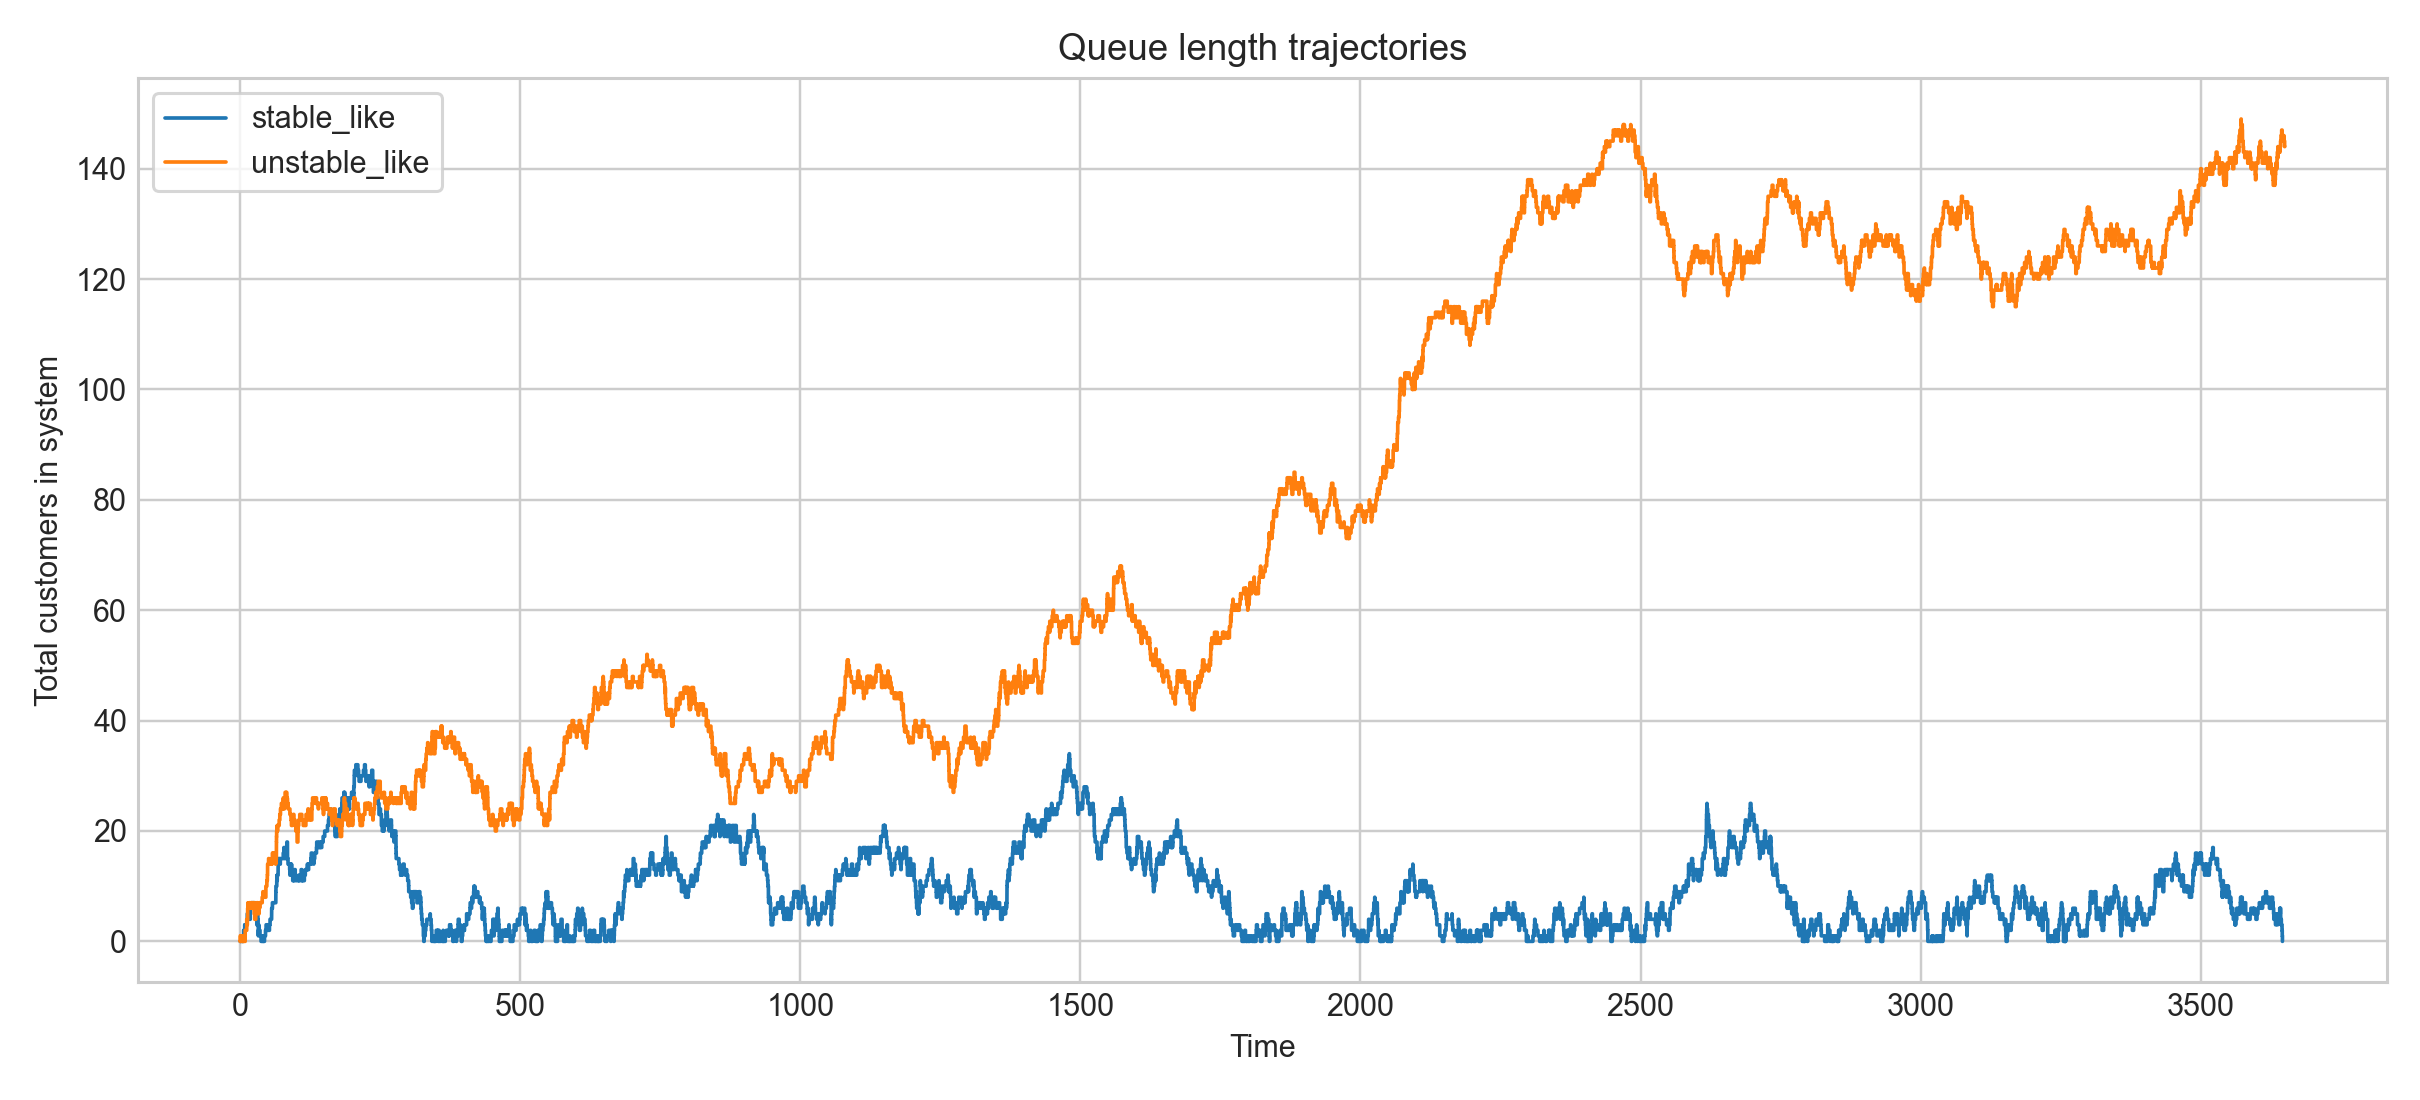
\includegraphics[width=\textwidth]{../results/parameter_variants/original_notebook/stability_replication.png}

\column{0.42\textwidth}
\small
\begin{tabular}{@{}lcc@{}}
\toprule
Variant & Stable case $p$ & Unstable case $p$ \\
\midrule
Paper text & 0.156 & 0.856 \\
Notebook & 0.00385 & 0.864 \\
\bottomrule
\end{tabular}

\vspace{0.8em}
\begin{block}{Interpretation}
The stable/nonstationary contrast is reproduced under the original-notebook switching rates. The paper-text stable case remains visually bounded but fails the $p<0.05$ ADF criterion.
\end{block}
\end{columns}
\end{frame}

\begin{frame}{Bounded Markov Approximation}
\begin{columns}[T]
\column{0.58\textwidth}
\centering
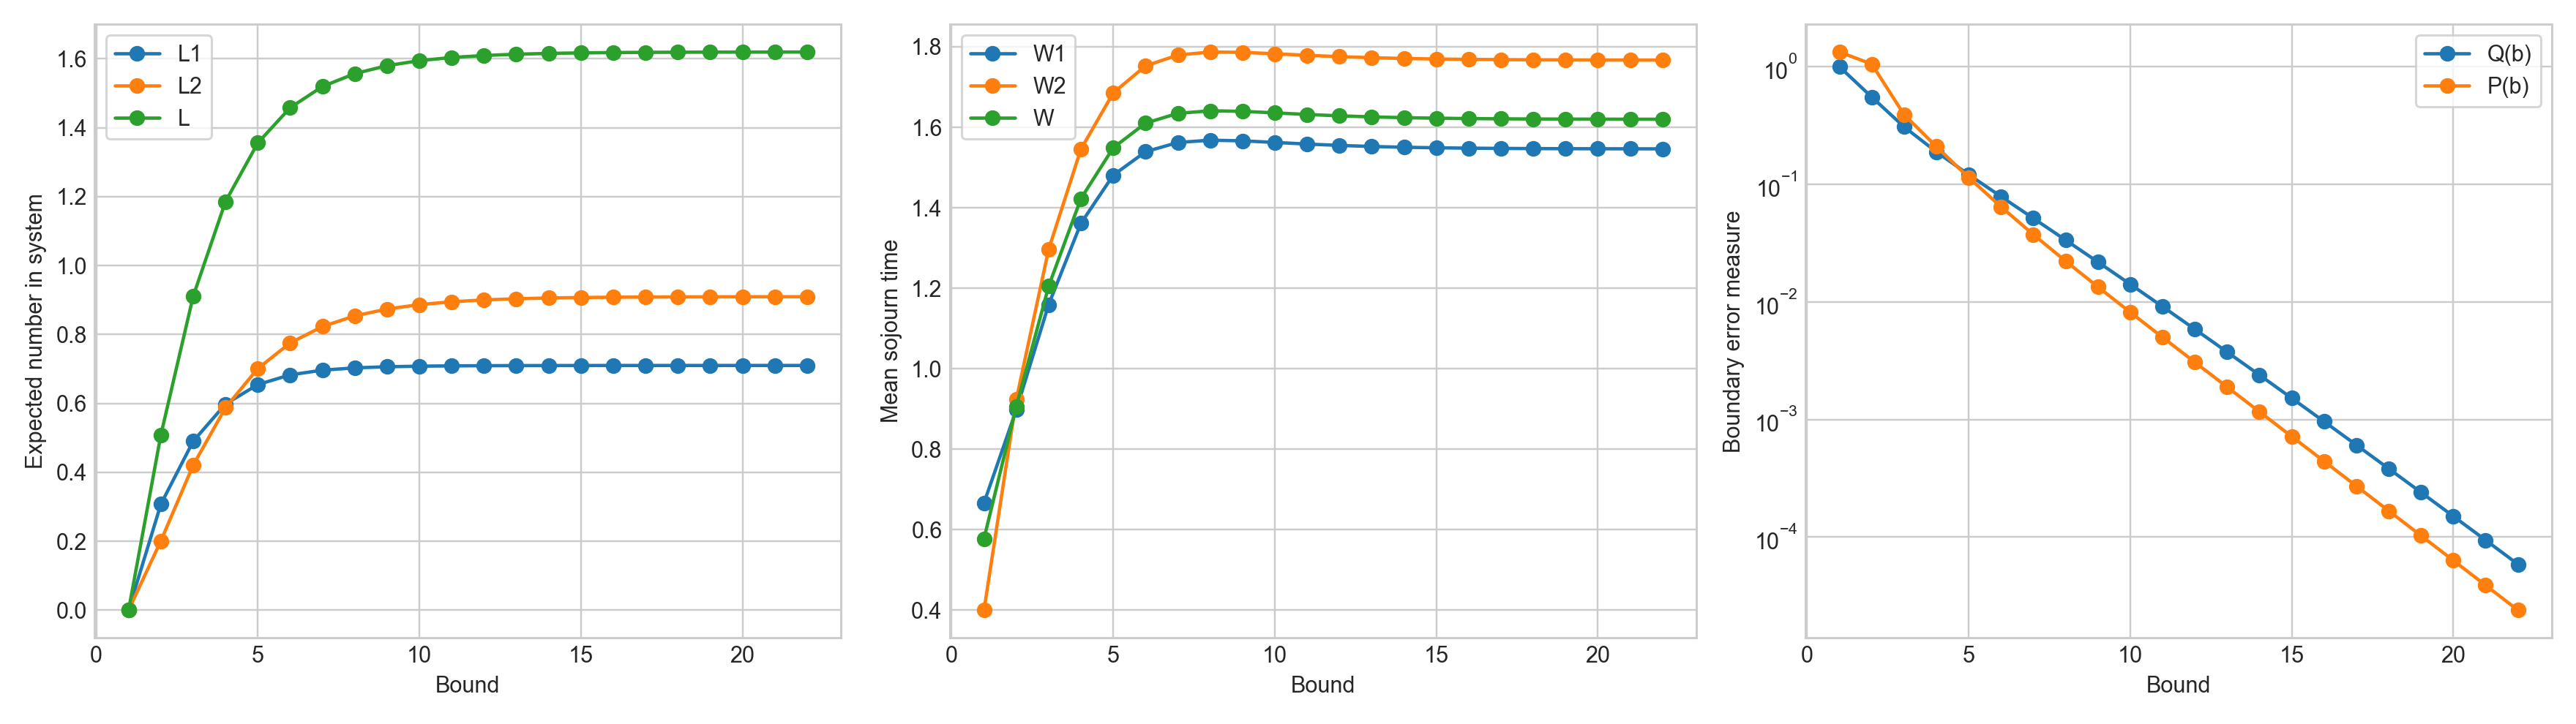
\includegraphics[width=\textwidth]{../results/parameter_variants/paper_text/bounded_markov_replication.png}

\column{0.42\textwidth}
\small
\begin{tabular}{@{}lccc@{}}
\toprule
Variant, $b=22$ & $L$ & $W$ & $Q(b)$ \\
\midrule
Paper text & 1.620 & 1.620 & $5.88{\times}10^{-5}$ \\
Notebook & 1.916 & 1.916 & $7.61{\times}10^{-5}$ \\
\bottomrule
\end{tabular}

\vspace{0.8em}
\begin{block}{Interpretation}
This is the strongest replication result. Truncation error becomes small in both parameter variants, and $L$ and $W$ stabilize as the bound grows.
\end{block}
\end{columns}
\end{frame}

\begin{frame}{Effect of Switching Matrix $H$}
\small
\begin{tabularx}{\textwidth}{@{}p{0.24\textwidth}ccccX@{}}
\toprule
Scenario & max $Q(16)$ & max $P(16)$ & $U_{\min}$ & $U_{\max}$ & Assessment \\
\midrule
A: prioritized slower & 0.0822 & 0.0120 & 1.704 & 7.927 &
\partialok: $P$ is within threshold, but $Q$ exceeds 0.012 at 181 grid points. \\
B: equal rates & 0.00753 & 0.00114 & 1.022 & 1.966 &
\ok: boundary checks pass across the grid. \\
C: prioritized faster & 0.0102 & 0.00152 & 0.521 & 2.257 &
\ok: boundary checks pass across the grid. \\
\bottomrule
\end{tabularx}

\vspace{0.8em}
\begin{block}{Interpretation}
The qualitative heatmap workflow is reproduced, but Scenario A should not be described as satisfying the paper's stated boundary check.
\end{block}
\end{frame}

\begin{frame}{Markov Chain vs Simulation}
\small
\begin{columns}[T]
\column{0.52\textwidth}
\centering
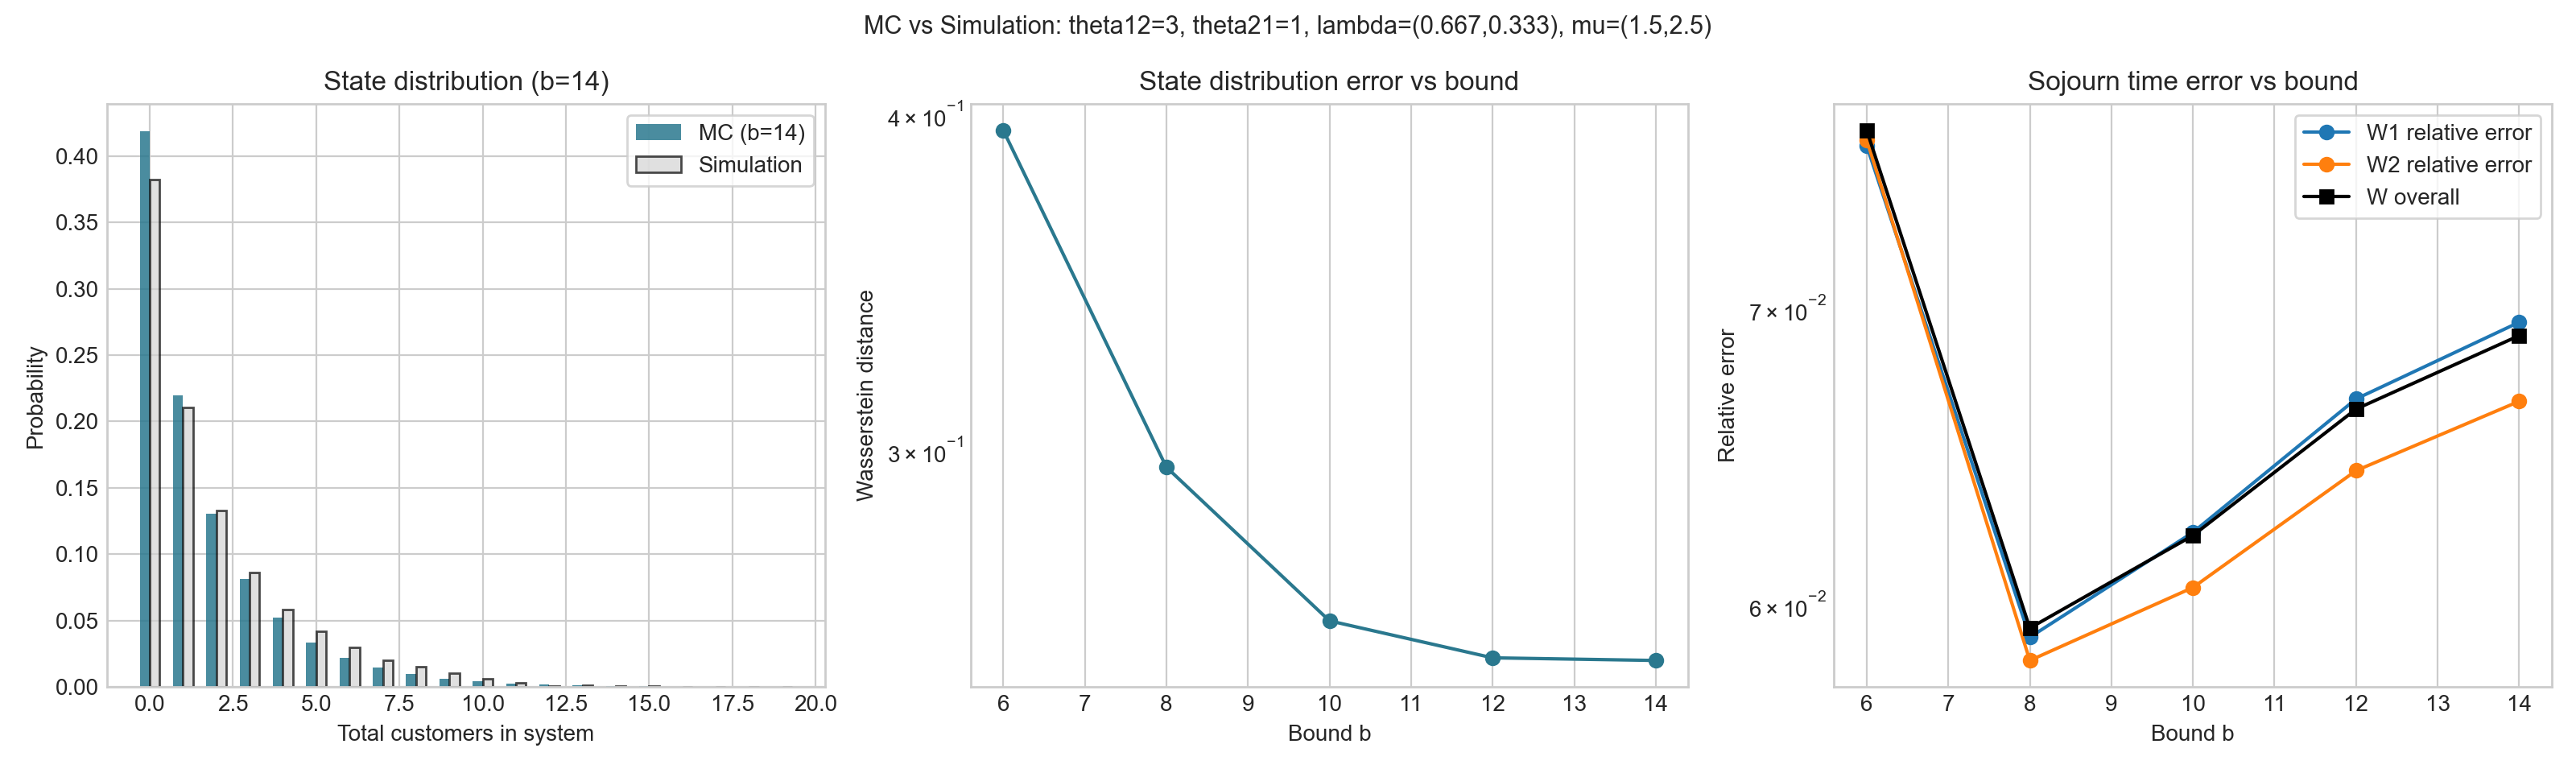
\includegraphics[width=\textwidth]{../results/parameter_variants/paper_text/mc_vs_sim_comparison.png}

\column{0.48\textwidth}
\begin{tabular}{@{}lcc@{}}
\toprule
Variant & W-error range & State-W range \\
\midrule
Paper text & 5.93--7.68\% & 0.251--0.395 \\
Notebook & 4.43--6.29\% & 0.104--0.308 \\
\bottomrule
\end{tabular}

\vspace{0.8em}
\begin{block}{Interpretation}
The validation is directionally reasonable, especially for state distributions, but the simulation horizon is short relative to the paper-scale long run.
\end{block}
\end{columns}
\end{frame}

\begin{frame}{Sojourn-Time Variance}
\begin{columns}[T]
\column{0.5\textwidth}
\centering
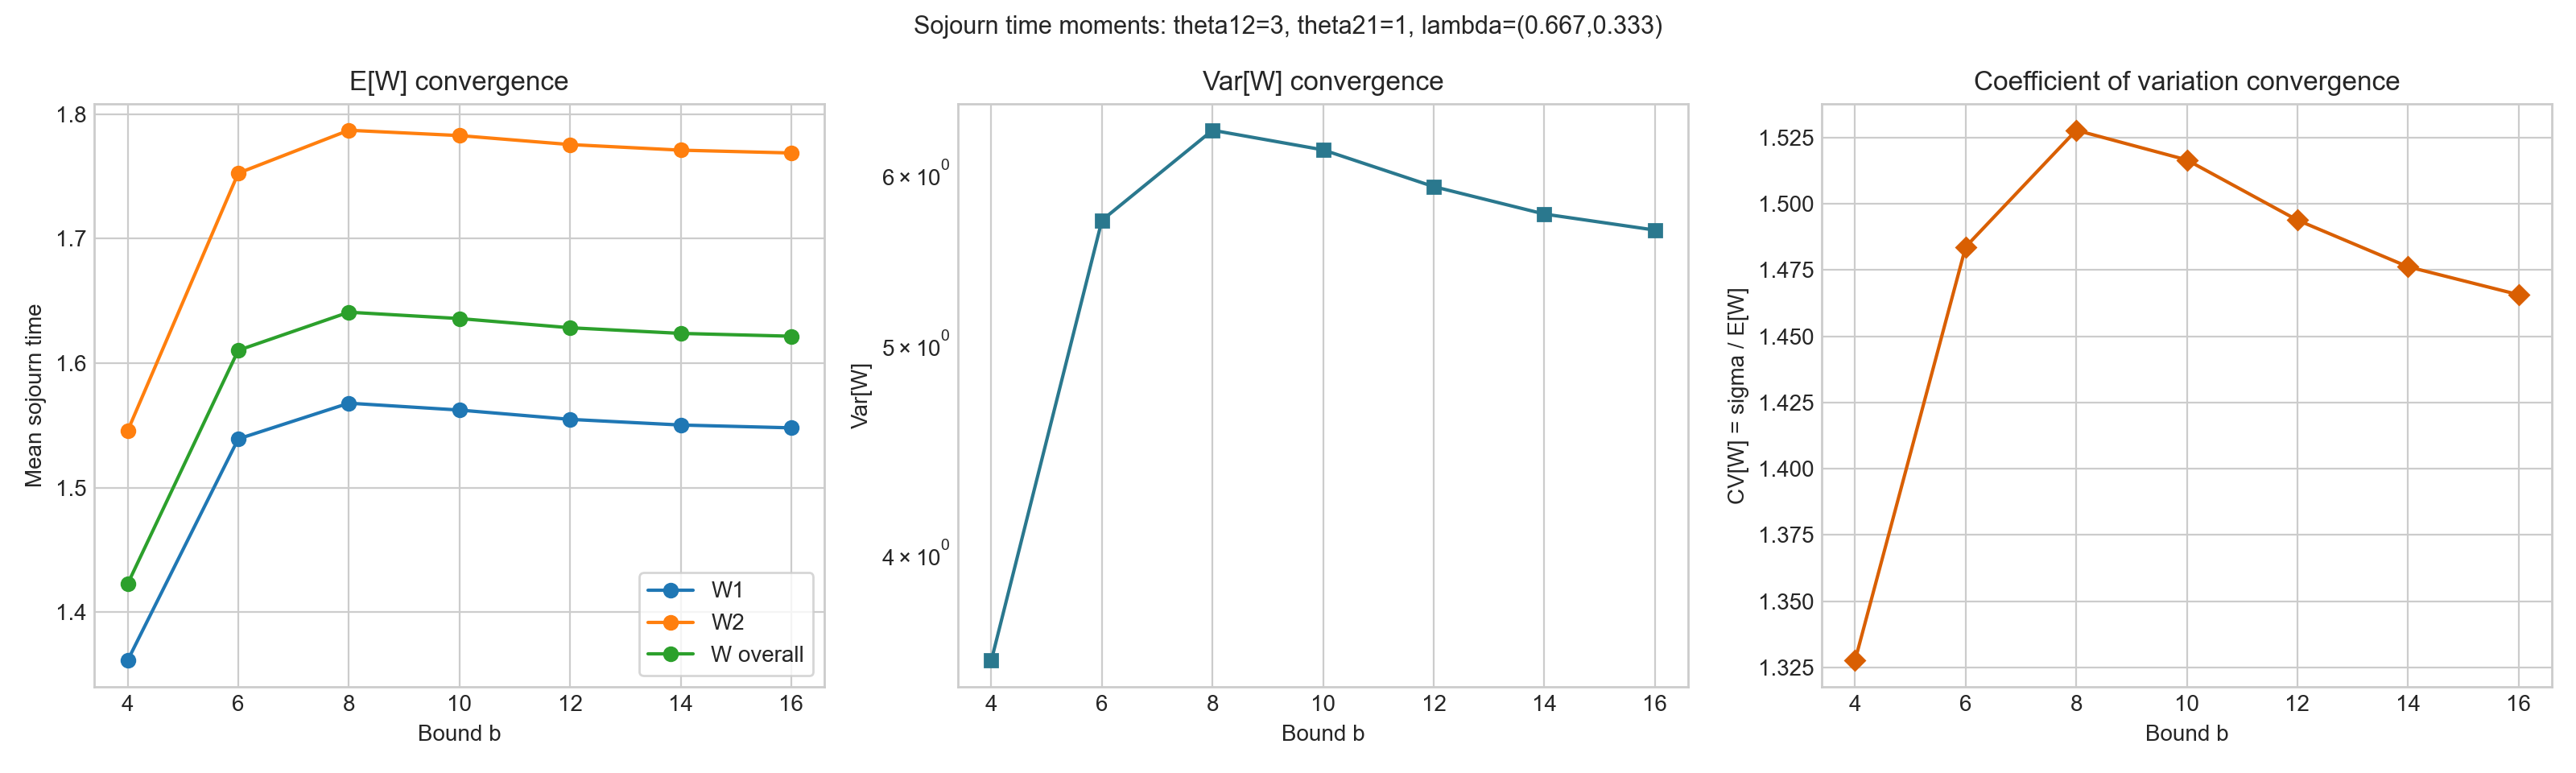
\includegraphics[width=\textwidth]{../results/parameter_variants/paper_text/sojourn_variance_convergence.png}

\column{0.5\textwidth}
\small
\begin{tabular}{@{}lccc@{}}
\toprule
Variant & $b$ & $W$ & Var$(W)$ \\
\midrule
Paper text & 16 & 1.622 & 5.649 \\
Notebook & 16 & 1.918 & 7.231 \\
\bottomrule
\end{tabular}

\vspace{0.8em}
\begin{block}{Interpretation}
The second-moment computation is internally consistent and useful. It should be presented as part reproduction of the absorbing-chain moment formulas plus additional visualization.
\end{block}
\end{columns}
\end{frame}

\begin{frame}{Extension: Fine-Grid Calibration}
\begin{columns}[T]
\column{0.52\textwidth}
\centering

\includegraphics[width=\textwidth]{extension_calibration_heatmap.png}

\column{0.48\textwidth}
\small
\begin{tabular}{@{}lccc@{}}
\toprule
Criterion & Point & W & MAPE \\
\midrule
Best calibration loss & $(3,2)$ & 2.657 & 0.179 \\
Best Wasserstein & $(1,2)$ & 2.576 & 0.285 \\
Best MAPE & $(3.5,2)$ & 3.368 & 0.108 \\
Paper point & $(3,1)$ & 3.977 & 0.518 \\
\bottomrule
\end{tabular}

\vspace{0.8em}
\begin{block}{Interpretation}
The composite loss is useful for screening the calibration landscape, but it is not a paper metric and is not normalized. It supports sensitivity analysis, not a definitive claim.
\end{block}
\end{columns}
\end{frame}

\begin{frame}{Main Takeaways}
\small
\begin{block}{What worked}
\begin{itemize}
  \item The repository now produces a complete, auditable result set for all implemented scripts.
  \item Bounded Markov convergence is robust under both parameter variants.
  \item The original-notebook stability experiment reproduces the expected split.
  \item The extension analyses are reasonable when clearly labeled as exploratory.
\end{itemize}
\end{block}

\begin{block}{What needs caution}
\begin{itemize}
  \item Fig.\ 5 does not confirm $(\theta_{12},\theta_{21})=(3,1)$ as the unique or best fit.
  \item Paper-text stability and Scenario A effect-of-$H$ boundary checks are not fully reproduced.
  \item MC-vs-sim validation needs longer simulation and confidence intervals before stronger claims.
\end{itemize}
\end{block}
\end{frame}

\begin{frame}
\begin{center}
{\Large \textbf{Thank you}}\\[1.5em]
{\small Questions and discussion}
\end{center}
\end{frame}

\end{document}
